%%%%%%%%%%%%%%%%%%%%%%%%%%%%%%%%%%%%%%%%%
% Beamer Presentation
% LaTeX Template
% Version 1.0 (10/11/12)
%
% This template has been downloaded from:
% http://www.LaTeXTemplates.com
%
% License:
% CC BY-NC-SA 3.0 (http://creativecommons.org/licenses/by-nc-sa/3.0/)
%
%%%%%%%%%%%%%%%%%%%%%%%%%%%%%%%%%%%%%%%%%

%----------------------------------------------------------------------------------------
%	PACKAGES AND THEMES
%----------------------------------------------------------------------------------------

\documentclass{beamer}

\mode<presentation> {

% The Beamer class comes with a number of default slide themes
% which change the colors and layouts of slides. Below this is a list
% of all the themes, uncomment each in turn to see what they look like.

%\usetheme{default}
%\usetheme{AnnArbor}
%\usetheme{Antibes}
%\usetheme{Bergen}
%\usetheme{Berkeley}
%\usetheme{Berlin}
%\usetheme{Boadilla}
%\usetheme{CambridgeUS}
%\usetheme{Copenhagen}
\usetheme{Darmstadt}
%\usetheme{Dresden}
%\usetheme{Frankfurt}
%\usetheme{Goettingen}
%\usetheme{Hannover}
%\usetheme{Ilmenau}
%\usetheme{JuanLesPins}
%\usetheme{Luebeck}
%\usetheme{Madrid}
%\usetheme{Malmoe}
%\usetheme{Marburg}
%\usetheme{Montpellier}
%\usetheme{PaloAlto}
%\usetheme{Pittsburgh}
%\usetheme{Rochester}
%\usetheme{Singapore}
%\usetheme{Szeged}
%\usetheme{Warsaw}

% As well as themes, the Beamer class has a number of color themes
% for any slide theme. Uncomment each of these in turn to see how it
% changes the colors of your current slide theme.

%\usecolortheme{albatross}
%\usecolortheme{beaver}
%\usecolortheme{beetle}
%\usecolortheme{crane}
%\usecolortheme{dolphin}
%\usecolortheme{dove}
%\usecolortheme{fly}
%\usecolortheme{lily}
%\usecolortheme{orchid}
%\usecolortheme{rose}
%\usecolortheme{seagull}
%\usecolortheme{seahorse}
\usecolortheme{whale}
%\usecolortheme{wolverine}

%\setbeamertemplate{footline} % To remove the footer line in all slides uncomment this line
%\setbeamertemplate{footline}[page number] % To replace the footer line in all slides with a simple slide count uncomment this line
\addtobeamertemplate{navigation symbols}{}{%
    \usebeamerfont{footline}%
    \usebeamercolor[fg]{footline}%
    \hspace{1em}%
    \insertframenumber/\inserttotalframenumber
}


   
%\setbeamertemplate{navigation symbols}{} % To remove the navigation symbols from the bottom of all slides uncomment this line
}
\usepackage[utf8]{inputenc}
\usepackage[english, greek]{babel}
\usepackage{alphabeta}
\usepackage{amsmath}
\usepackage{mathtools}
\DeclarePairedDelimiter{\abs}{\lvert}{\rvert}
\DeclarePairedDelimiter\floor{\lfloor}{\rfloor}
\usepackage{graphicx} % Allows including images
\usepackage{booktabs} % Allows the use of \toprule, \midrule and \bottomrule in tables
\usepackage{hyperref}

%----------------------------------------------------------------------------------------
%	TITLE PAGE
%----------------------------------------------------------------------------------------

\title[\textlatin{Travelling Salesman Problem (TSP)}] {\textlatin{Travelling Salesman Problem (TSP)}}
\subtitle{Prohgm'ena J'emata Algor'ijmwn}
% The short title appears at the bottom of every slide, the full title is only on the title page

\author{Jeod'wra Panag'ea  1115201400135} % Your name
\institute[EKPA] % Your institution as it will appear on the bottom of every slide, may be shorthand to save space
{
Εjnik'o kai Kapodistriak'o Panepist'hmio Ajhn'wn \\ % Your institution for the title page
\medskip
\textit{ } % Your email address
}
\date{M'aios 2021} % Date, can be changed to a custom date

\begin{document}

\begin{frame}
\titlepage % Print the title page as the first slide
\end{frame}

\section{Eisagwg'h}
\frame{\frametitle{Εισαγωγή}
Βασικά σημεία της σημερινής παρουσίασης:
\begin{itemize}
    \item Ορισμός \textlatin{TSP}
    \item \textlatin{Αρχικές ιδέες επίλυσης του Προβλήματος}
    \item \textlatin{ΝP-complete} και Αναγωγή
    \item Προσεγγιστικός Αλγόριθμος
\end{itemize}
}
\frame{\frametitle{'Ena gr'hgoro skon'aki...}
\begin{itemize}
    \item \textbf{Κύκλος \textlatin{Euler}:} Κύκλος που επισκέπτεται όλες τις ακμές ακριβώς 1 φορά.
    \item \textbf{Κύκλος \textlatin{Hamilton:}} Κύκλος που επισκέπτεται όλες τις κορυφές ακριβώς 1 φορά. 
    \item \textbf{Κορυφή περιττού βαθμού:} Κορυφή με περιττό πλήθος ακμών
    \item \textbf{Κορυφή άρτιου βαθμού:} Κορυφή με άρτιο πλήθος ακμών
    \item \textbf{\textlatin{MST}:} Ένωση όλων των κορυφών με το ελάχιστο κόστος
    \item \textbf{Τέλειο ταίριασμα:} Κάθε κορυφή έχει ακριβώς 1 ακμή
    \item \textbf{Τριγωνική Ανισότητα:} Συντομότερη διαδρομή μεταξύ 2 κορυφών είναι η ακμή που τις ενώνει. 
\end{itemize}
}

\section{Orism'os}
\frame{\frametitle{Ορισμός \textlatin{TSP}}
\begin{block}{Το πρόβλημα}
Ένας πωλητής πρέπει να επισκεφθεί όλες τις πόλεις σε ένα δίκτυο πόλεων ακριβώς 1 φορά, κάνοντας το μικρότερο ταξίδι. 
\end{block}
\pause
\begin{block}{Στόχος}
Εύρεση μονοπατιού/περιοδείας που περιλαμβάνει όλες τις πόλεις από 1 φορά κι έχει ελάχιστο μήκος.  
\end{block} 
\pause
\begin{block}{Τα δεδομένα μας}
\begin{itemize}
    \item Πόλεις $1, 2,\ldots, n$ και αποστάσεις (πόσες?)
    \item Πωλητής ξεκινάει από την 1
    \item Προϋπολογισμός \textlatin{b}
\end{itemize}

\end{block}
}

\frame{\frametitle{Ορισμός \textlatin{TSP}}
\begin{center}
    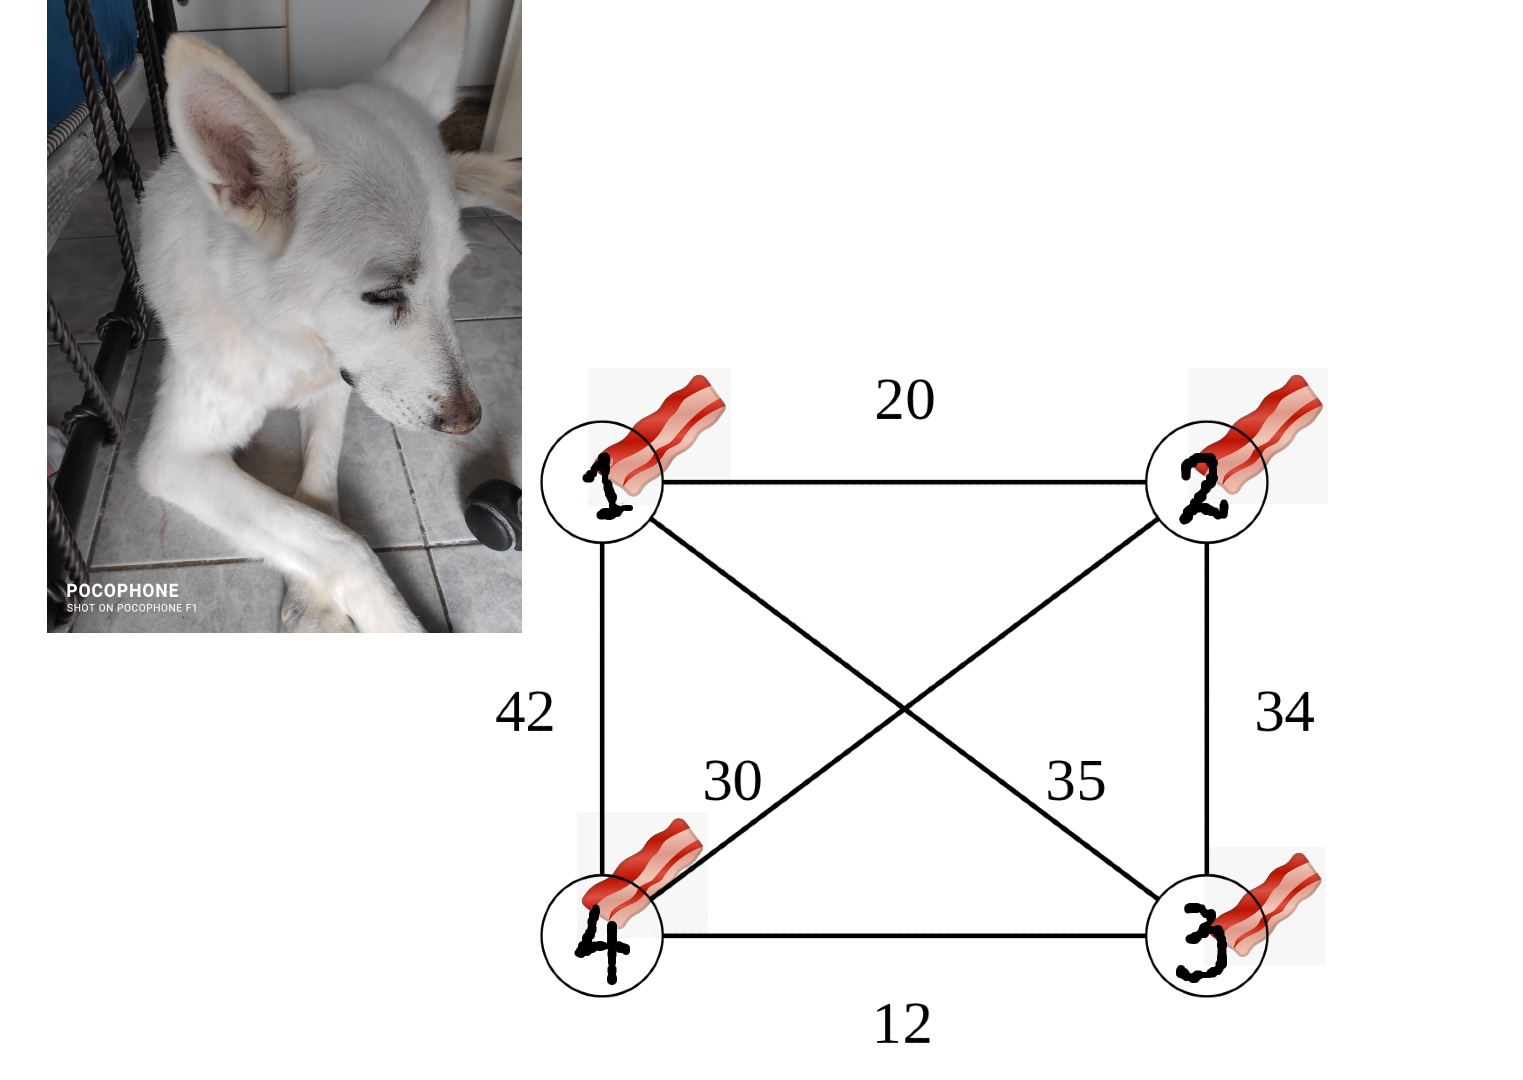
\includegraphics[width=10cm]{Rea.jpg}
\end{center}
}

\section{Id'ees Ep'ilushs}
\frame{ \frametitle{Ιδέες Επίλυσης}
\begin{center}
    \textbf{ \textlatin{Bruteforce}}
\end{center}
Βρίσκουμε όλες τις δυνατές περιοδείες και παίρνουμε την καλύτερη.
\begin{itemize}
    \item Πλήθος δυνατών επιλογών: $(n-1)!$
    \item Πολυπλοκότητα: $\mathcal{O}(n!)$
\end{itemize}
\begin{center}
    
\includegraphics[width=5cm]{itachi.jpeg}
\end{center}

}

\frame{ \frametitle{Ιδέες Επίλυσης}
\begin{center}
\textbf{Δυναμικός Προγραμματισμός} \\ ΠΟΛΥ ταχύτερη λύση αλλά... \\ ακόμα δεν είναι πολυωνυμική!
\end{center}
\pause
\begin{block}{Το υποπρόβλημα}
Για ένα υποσύνολο πόλεων $ S \subseteq {1,2,...,n}$ το οποίο περιλαμβάνει την 1, και $j \in S$, έστω $C(S, j)$ το μήκος της συντομότερης διαδρομής η οποία επισκέπτεται κάθε κόμβο του $S$ μόνο μία φορά, ξεκινώντας από την 1 και καταλήγοντας στη $j$. 
\end{block}
}

\section{\textlatin{NP-complete} kai Anagwg'h}
\begin{frame}\frametitle{\textlatin{NP-complete} kai Anagwg'h}
\begin{center}
\textbf{Τι γνωρίζουμε μέχρι στιγμής:}
\end{center}

\begin{itemize}
    \item N κορυφές, $\frac{n(n-1)}{2}$ αποστάσεις
    \item Ψάχνουμε περιοδεία, περνάει από κάθε πόλη 1 φορά, με κόστος $C \leq b$ $\Rightarrow$
    \item Θέλουμε μετάθεση των κορυφών ώστε:
    $$d_{1,2} + d_{2,3} + \ldots + d_{n,1} \leq b$$
\end{itemize}
\end{frame}

\begin{frame}\frametitle{\textlatin{NP-complete} kai Anagwg'h}
 \begin{block}{Pistopoihtik'o}
 Εξετάζει αν η περιοδεία περιλαμβάνει όλες τις πόλεις ακριβώς 1 φορά, προσθέτει τα κόστη κι αποφασίζει αν είναι μεγαλύτερο ή ίσο του \textlatin{b}.
 \end{block}

\end{frame}

\begin{frame}
    \begin{center}
    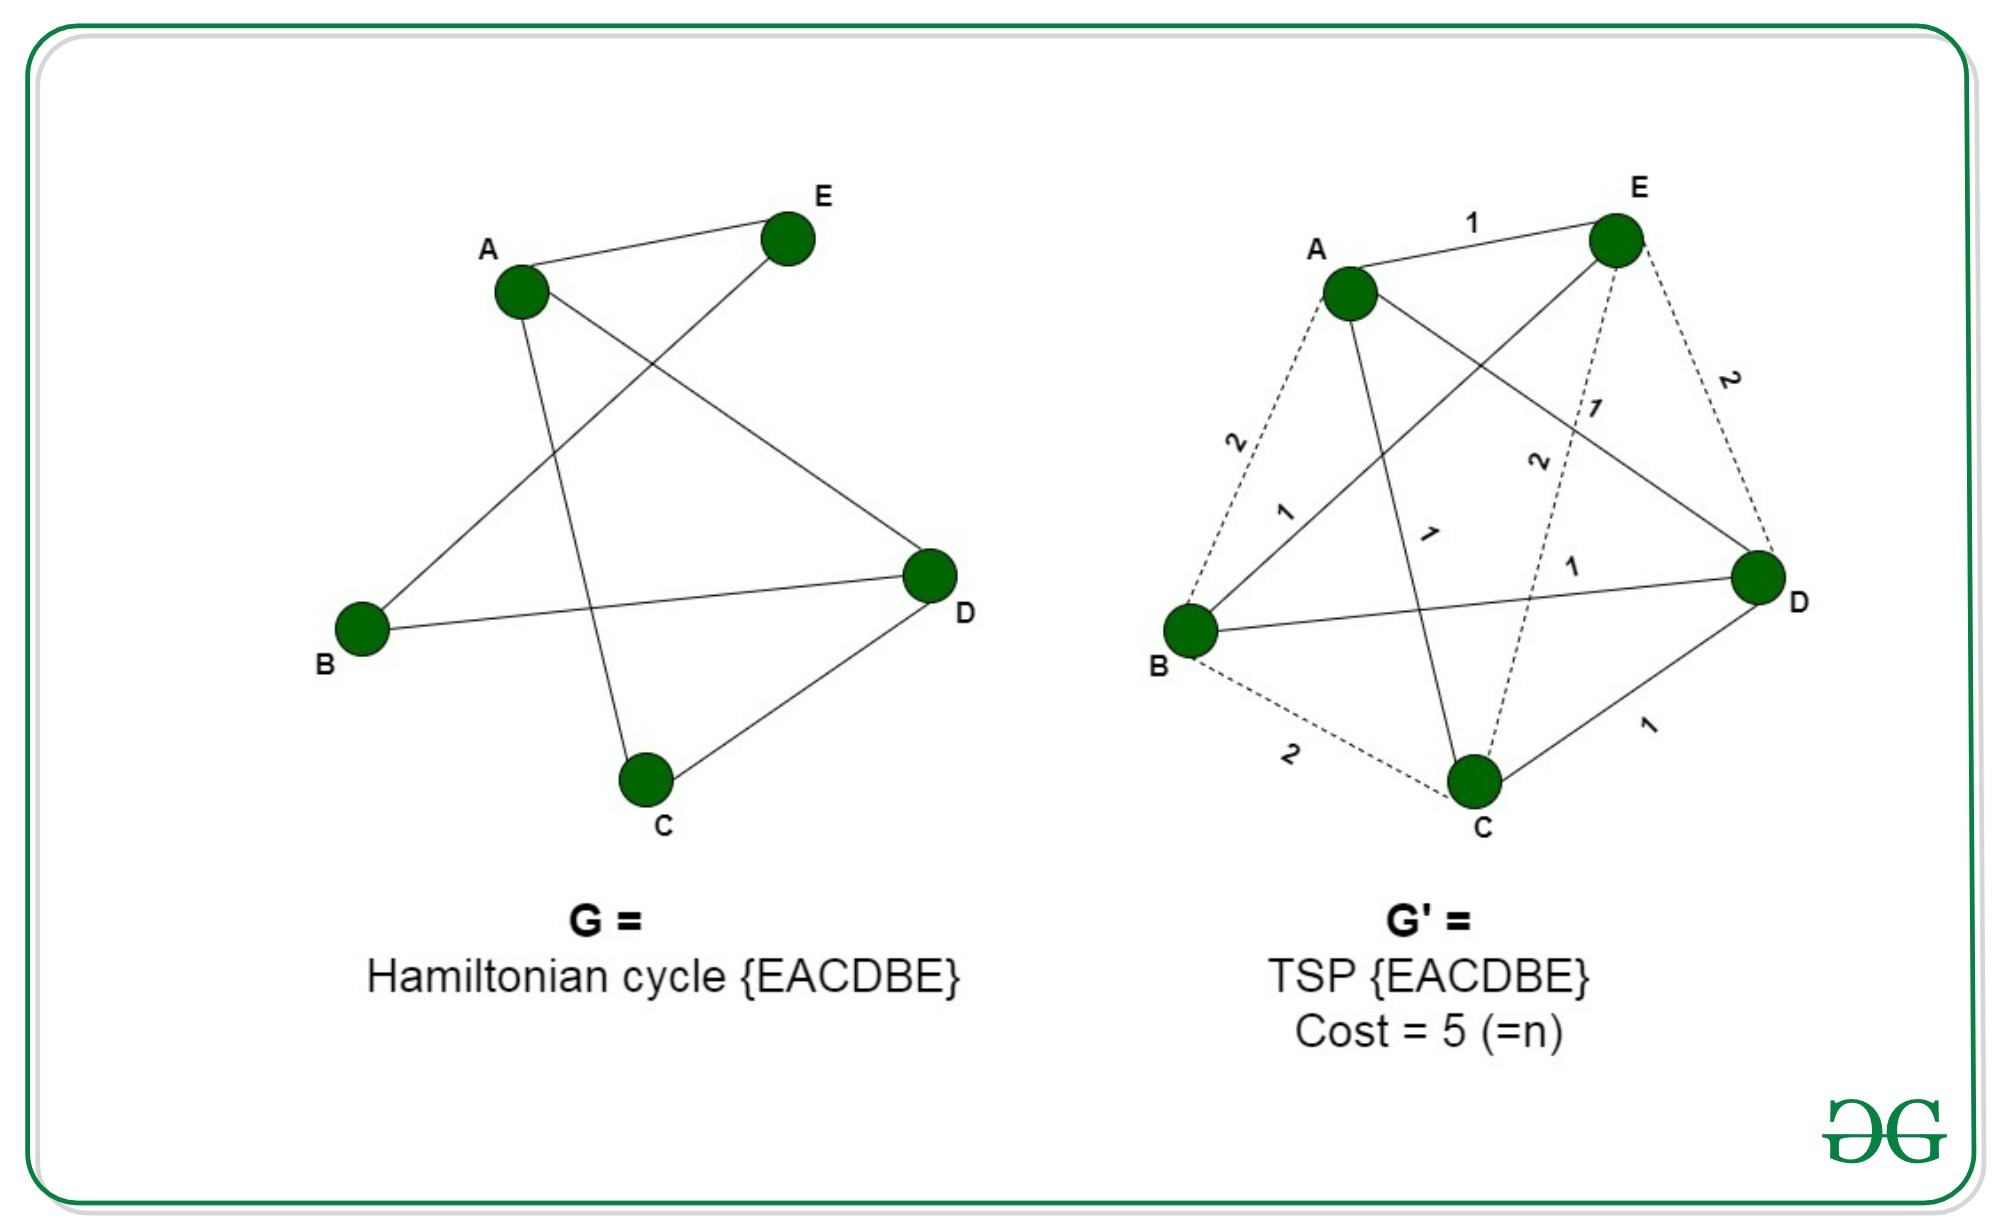
\includegraphics[width=\textwidth]{tsp1.jpg}
\end{center}
\end{frame}

\begin{frame}{\textlatin{NP-complete} kai Anagwg'h}
\textbf{Απόδειξη:}
\begin{itemize}
    \item Γράφημα $G$, κατασκευάζω στιγμιότυπο \textlatin{TSP}. Κόστος 1 αν $(u,v)$ υπάρχει, $1+α$ διαφορετικά, με $α>1$ 
    \item Προϋπολογισμός: $\abs V$
    \item Αν έχει κύκλο \textlatin{Hamilton}, τότε θα ειναι και η λύση του \textlatin{TSP}.
    \item Αν δεν έχει, τότε δεν υπάρχει και λύση. Φθηνότερη δυνατή θα έχει κόστος $n+α$
    
\end{itemize}
\begin{itemize}
    \item[1η περ:] $α=1$, \textlatin{Metric TSP} γιατί ισχύει η τριγωνική ανισότητα. 
    \item[2η περ:] Το $α$ αυθαίρετα μεγάλο. Τότε υπάρχει λύση με κόστος $\leq n$ ή όλες οι λύσεις είναι τουλ. $n+α$.
\end{itemize}

\end{frame}


\section{Προσεγγιστικός Αλγόριθμος}
\begin{frame}{\textlatin{Metric TSP 2-Προσεγγιστικός}}
\emph{Γνωρίζουμε κάποια εύκολη δομή που σχετίζεται με την καλύτερη περιήγηση του πωλητή?} \newline
Ναι! Τo \textlatin{MST} :) \newline \newline
Ισχύει ότι:
$$\text{κόστος } MST \leq \text{κόστος αυτής της διαδρομής} \leq \text{κόστος }  TSP$$
\end{frame}

\begin{frame}{\textlatin{Metric TSP 2-Προσεγγιστικός}}
\emph{Πώς θα χρησιμοποιήσουμε το $MST$?}
\begin{center}
    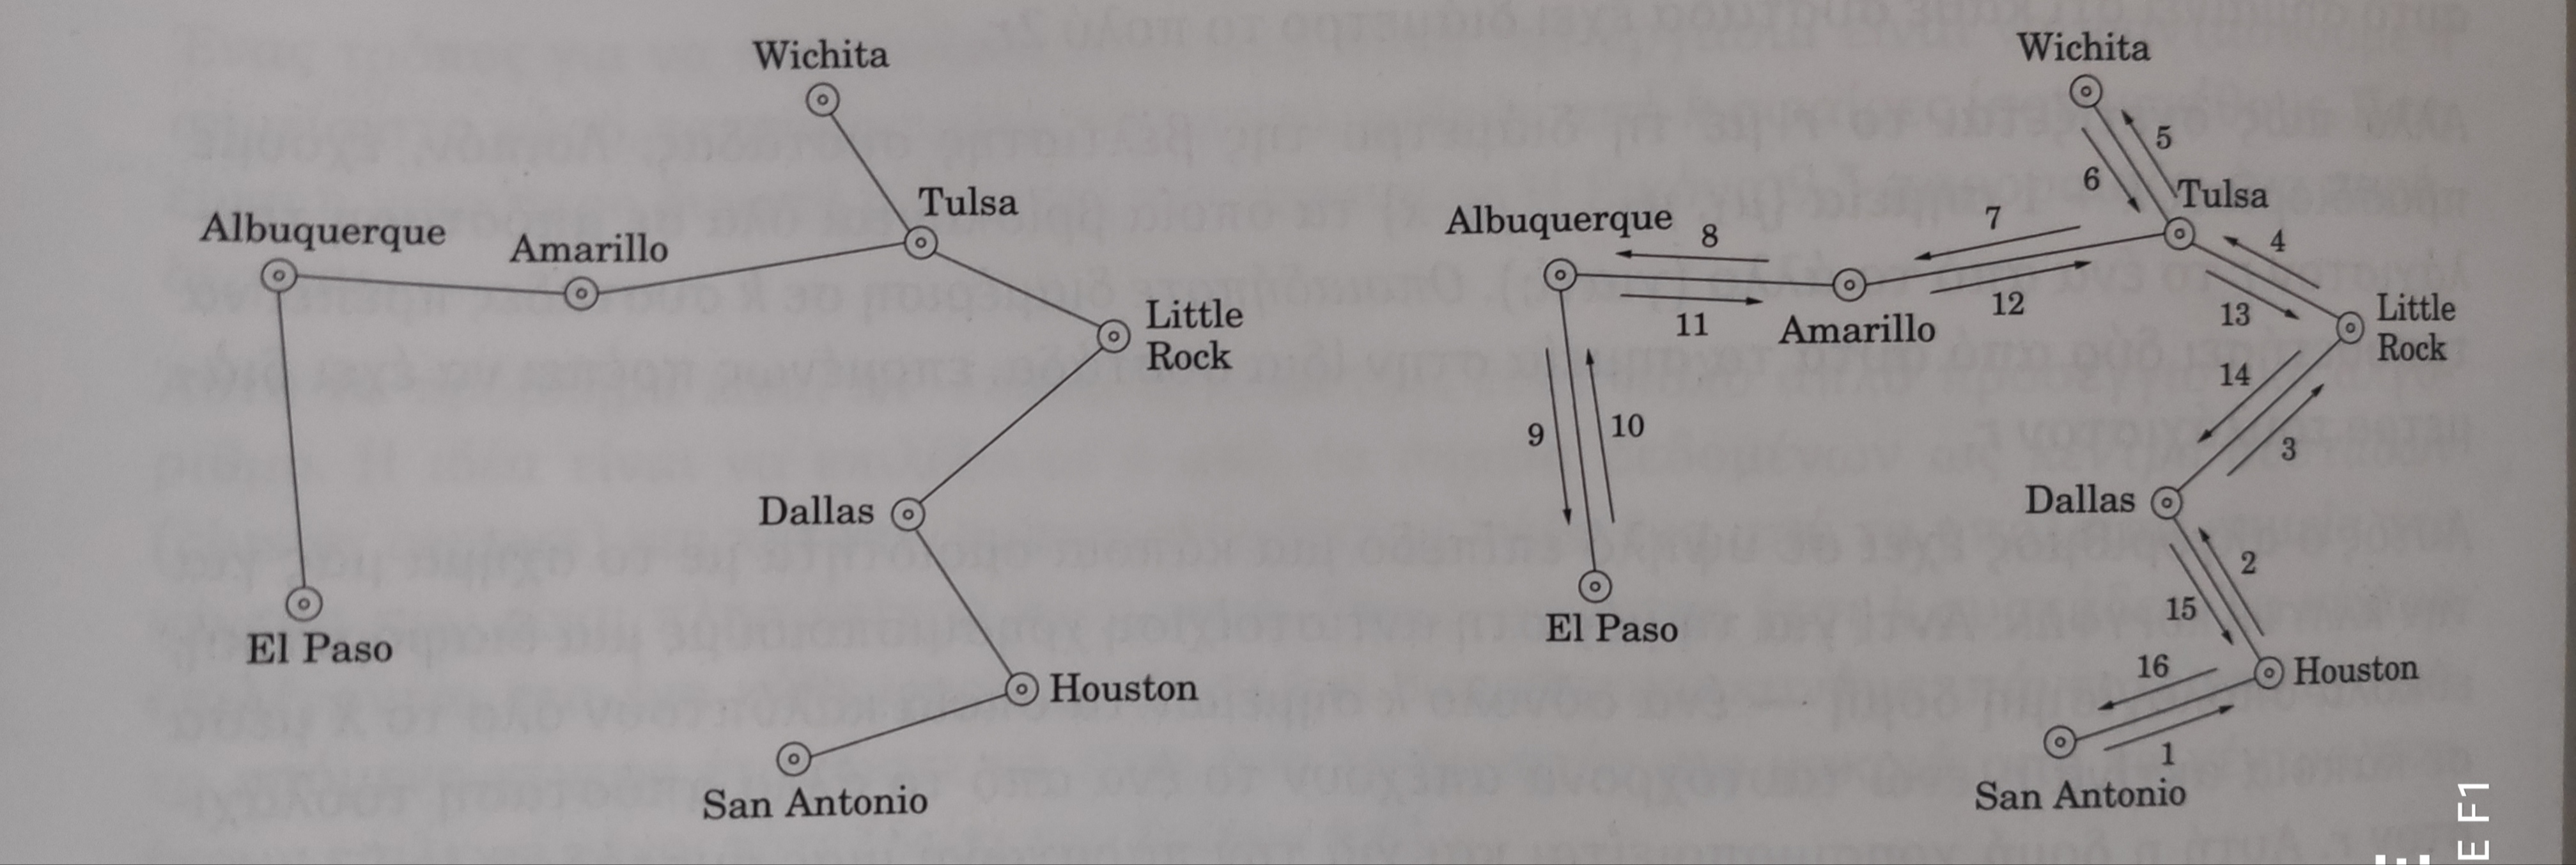
\includegraphics[width=10cm]{example.jpg}
\end{center}
Μήκος το πολύ διπλάσιο από το κόστος του $MST$ \newline ΑΛΛΑ επισκέπτεται κάποιες πόλεις πολλές φορές. Πώς το φτιάχνουμε?
\end{frame}

\begin{frame}{\textlatin{Metric TSP 2-Προσεγγιστικός}}
\emph{Διαδικασία:}
\begin{enumerate}
    \item Πλήρες γράφημα
    \item Δημιουργία \textlatin{MST}
    \item \textlatin{DFS} στο \textlatin{MST}
    \item Διαγραφή \textlatin{duplicates} από το \textlatin{output} της \textlatin{DFS}
\end{enumerate}

\begin{center}
    \includegraphics[width=5cm]{Στιγμιότυπο 2021-06-02, 13.40.38.png}
\end{center}

\end{frame}


\begin{frame}{\textlatin{Metric TSP} 3/2-Προσεγγιστικός}
    \emph{Βελτίωση λόγου προσέγγισης:}
    \begin{center}
        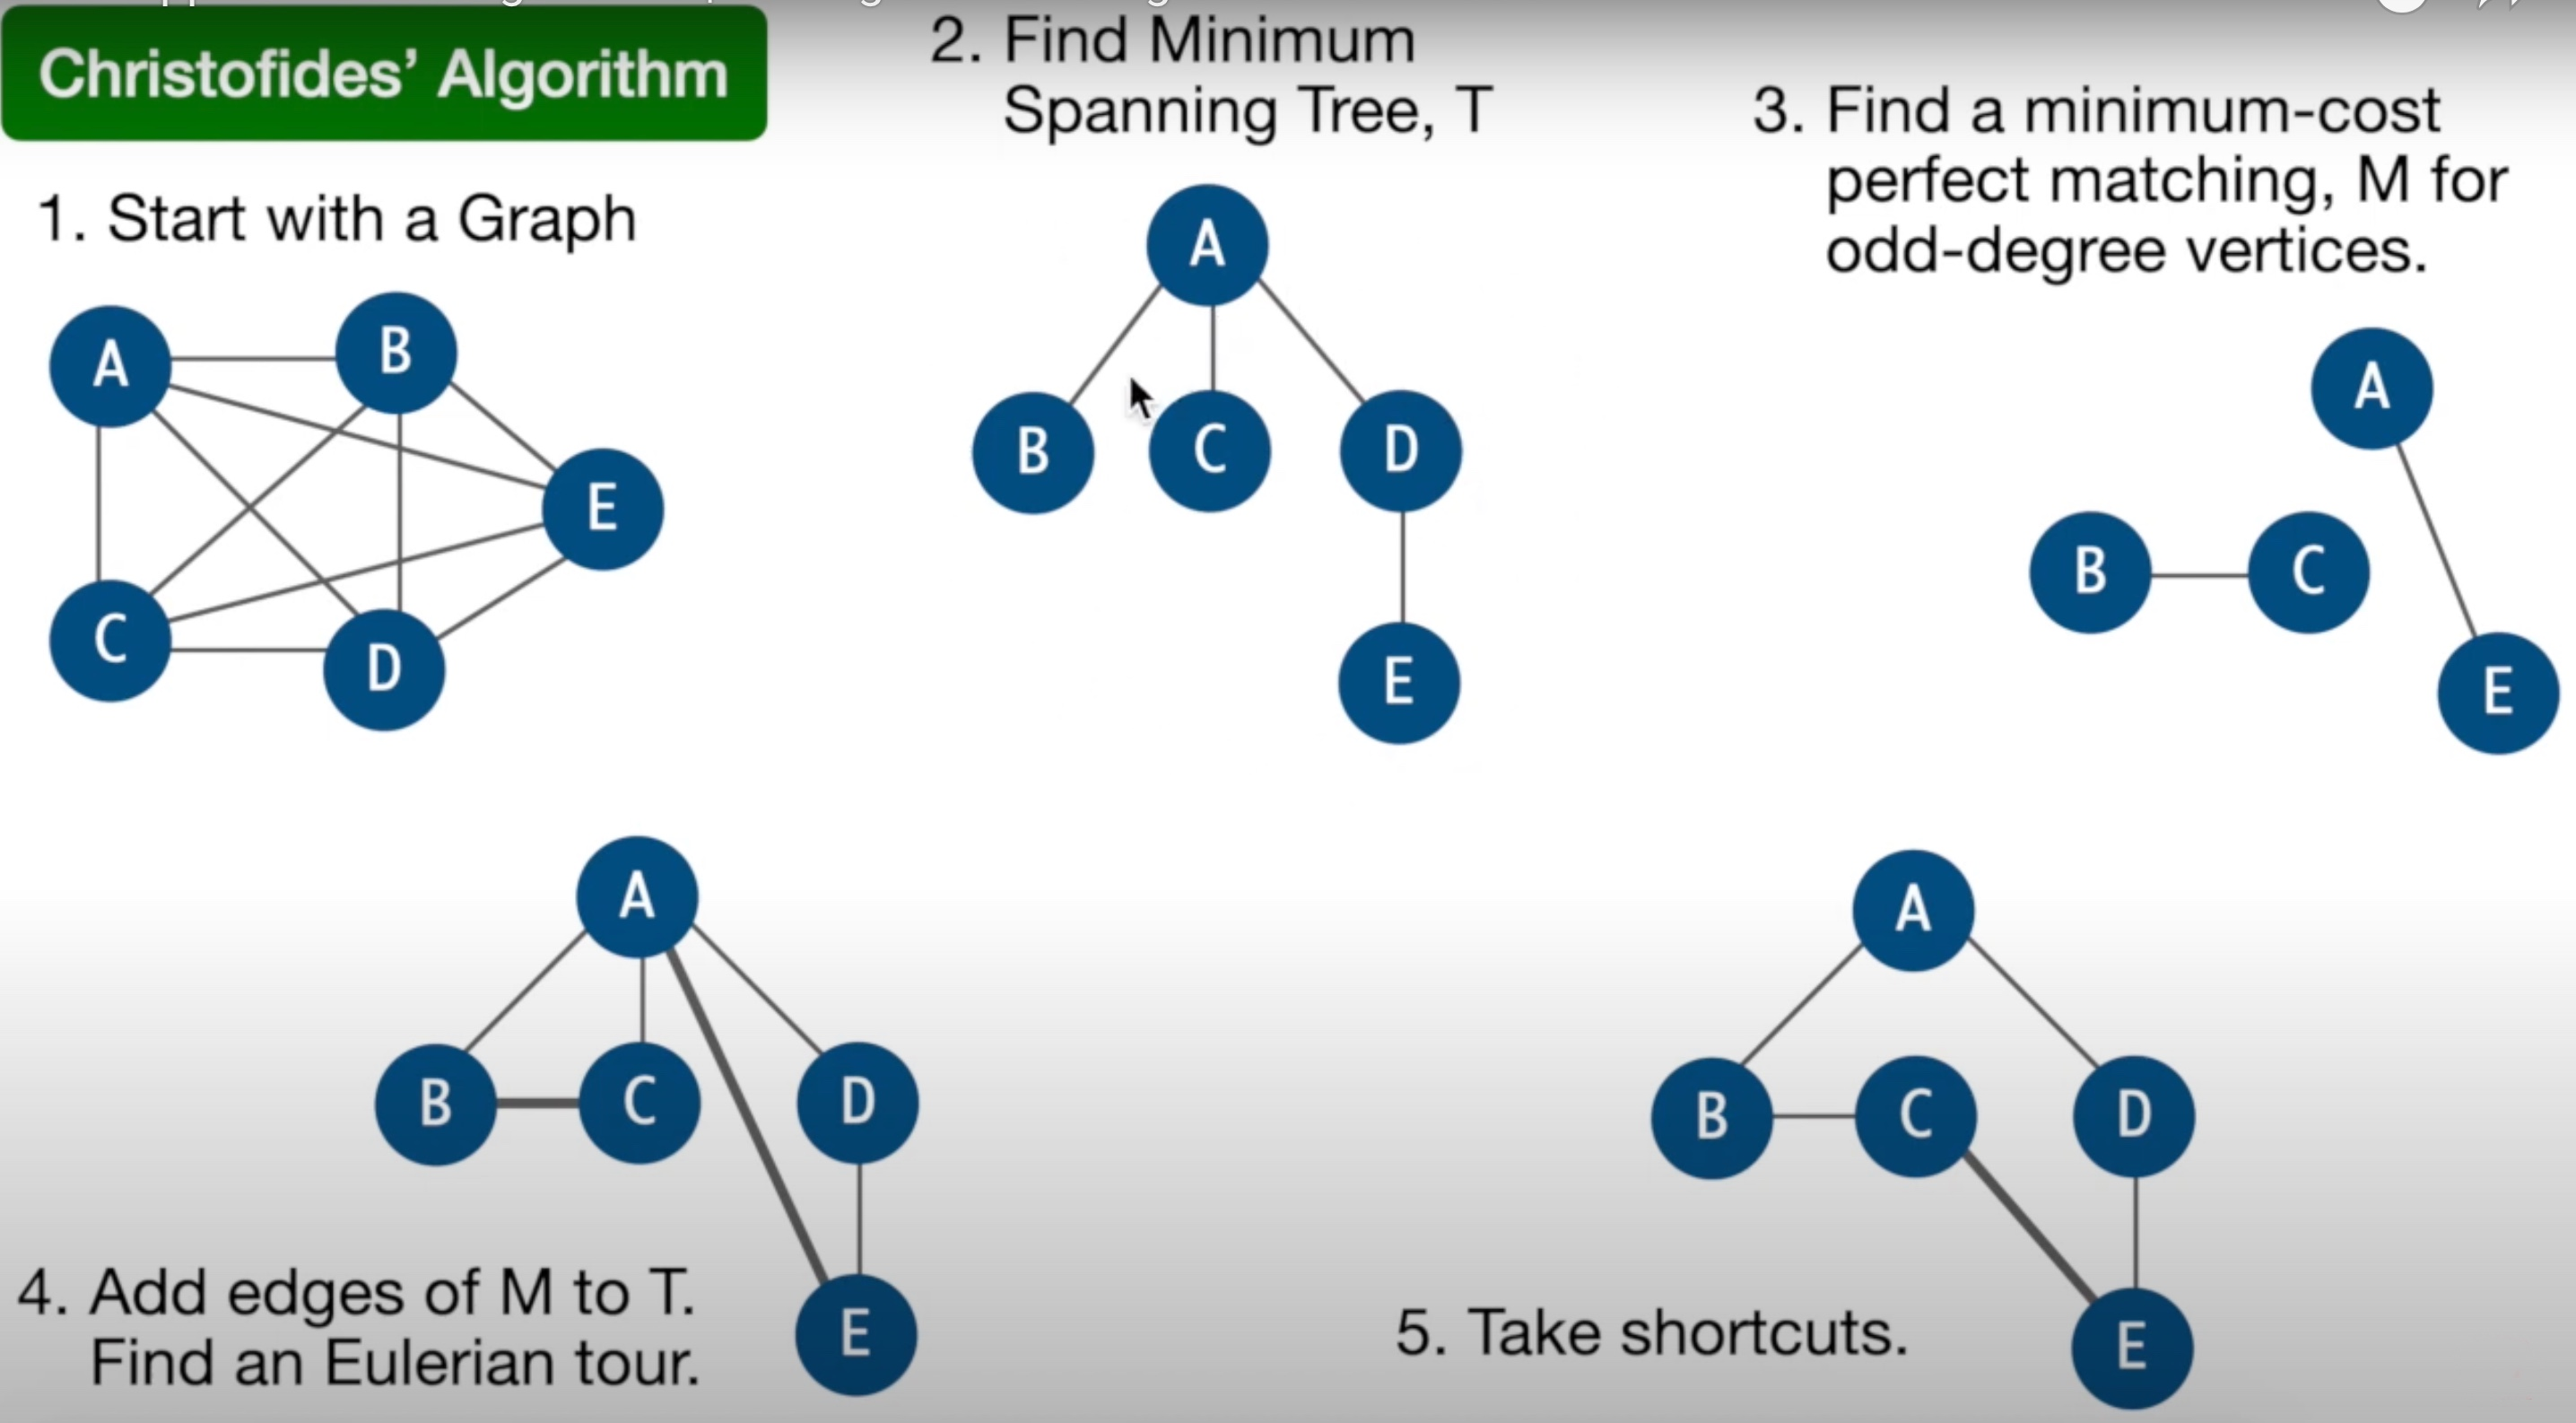
\includegraphics[width=\textwidth]{rec.jpg}
    \end{center}
\end{frame}

\begin{frame}{Γενικό \textlatin{TSP} και Προσεγγισιμότητα}
    Έστω αλγόριθμος $Α$ για το $TSP$ και $α_Α$ ο λόγος προσέγγισης. Από το πρόβλημα του κύκλου \textlatin{Hamilton}, φτιάχνω στιγμιότυπο για το \textlatin{TSP}.
    \begin{itemize}
        \item [1η περ:] Επιτυχία, περιήγηση το πολύ $n α_A$
        \item [2h περ:] Αποτυχία, περιήγηση τουλάχιστον $n α_A$
    \end{itemize}
    Άρα, σε πολυωνυμικό χρόνο μπορώ να προσδιορίσω αν το $G$ έχει κύκλο \textlatin{Hamilton} και αν τρέξουμε τη διαδικασία πολλές φορές (πολυωνυμικό πλήθος) θα βρούμε και τη διαδρομή. 
    \newline \newline
    Άρα: πολυωνυμικός αλγόριθμος για το NR-πλήρες πρόβλημα του κύκλου \textlatin{Hamilton}. 
    \begin{center}
    \textbf{MONO AN $P = NP$}
    \end{center}
  
\end{frame}


\begin{frame}{Αναφορές}
\begin{enumerate}
    \item Στοιχεία Θεωρίας Υπολογισμού - \textlatin{Harry R. Lewis}, Χρίστος Παπαδημητρίου, Εκδόσεις Κριτική
    \item \textlatin{Approximation Algorithms - Vazirani}, Εκδόσεις \textlatin{Springer}
    \item Αλγόριθμοι - \textlatin{Dasgupta}, Παπαδημητρίου, \textlatin{Vazirani}, Εκδόσεις Κλειδάριθμος
    \item Σχεδιασμός Αλγορίθμων - \textlatin{Kleinberg, Tardos}, Εκδόσεις Κλειδάριθμος 
    \item \href{http://www.cs.cornell.edu/courses/cs681/2007fa/Handouts/christofides.pdf}{\textlatin{Christofides' Algorithm}}
    
\end{enumerate}
    
\end{frame}


\begin{frame}
\begin{center}
    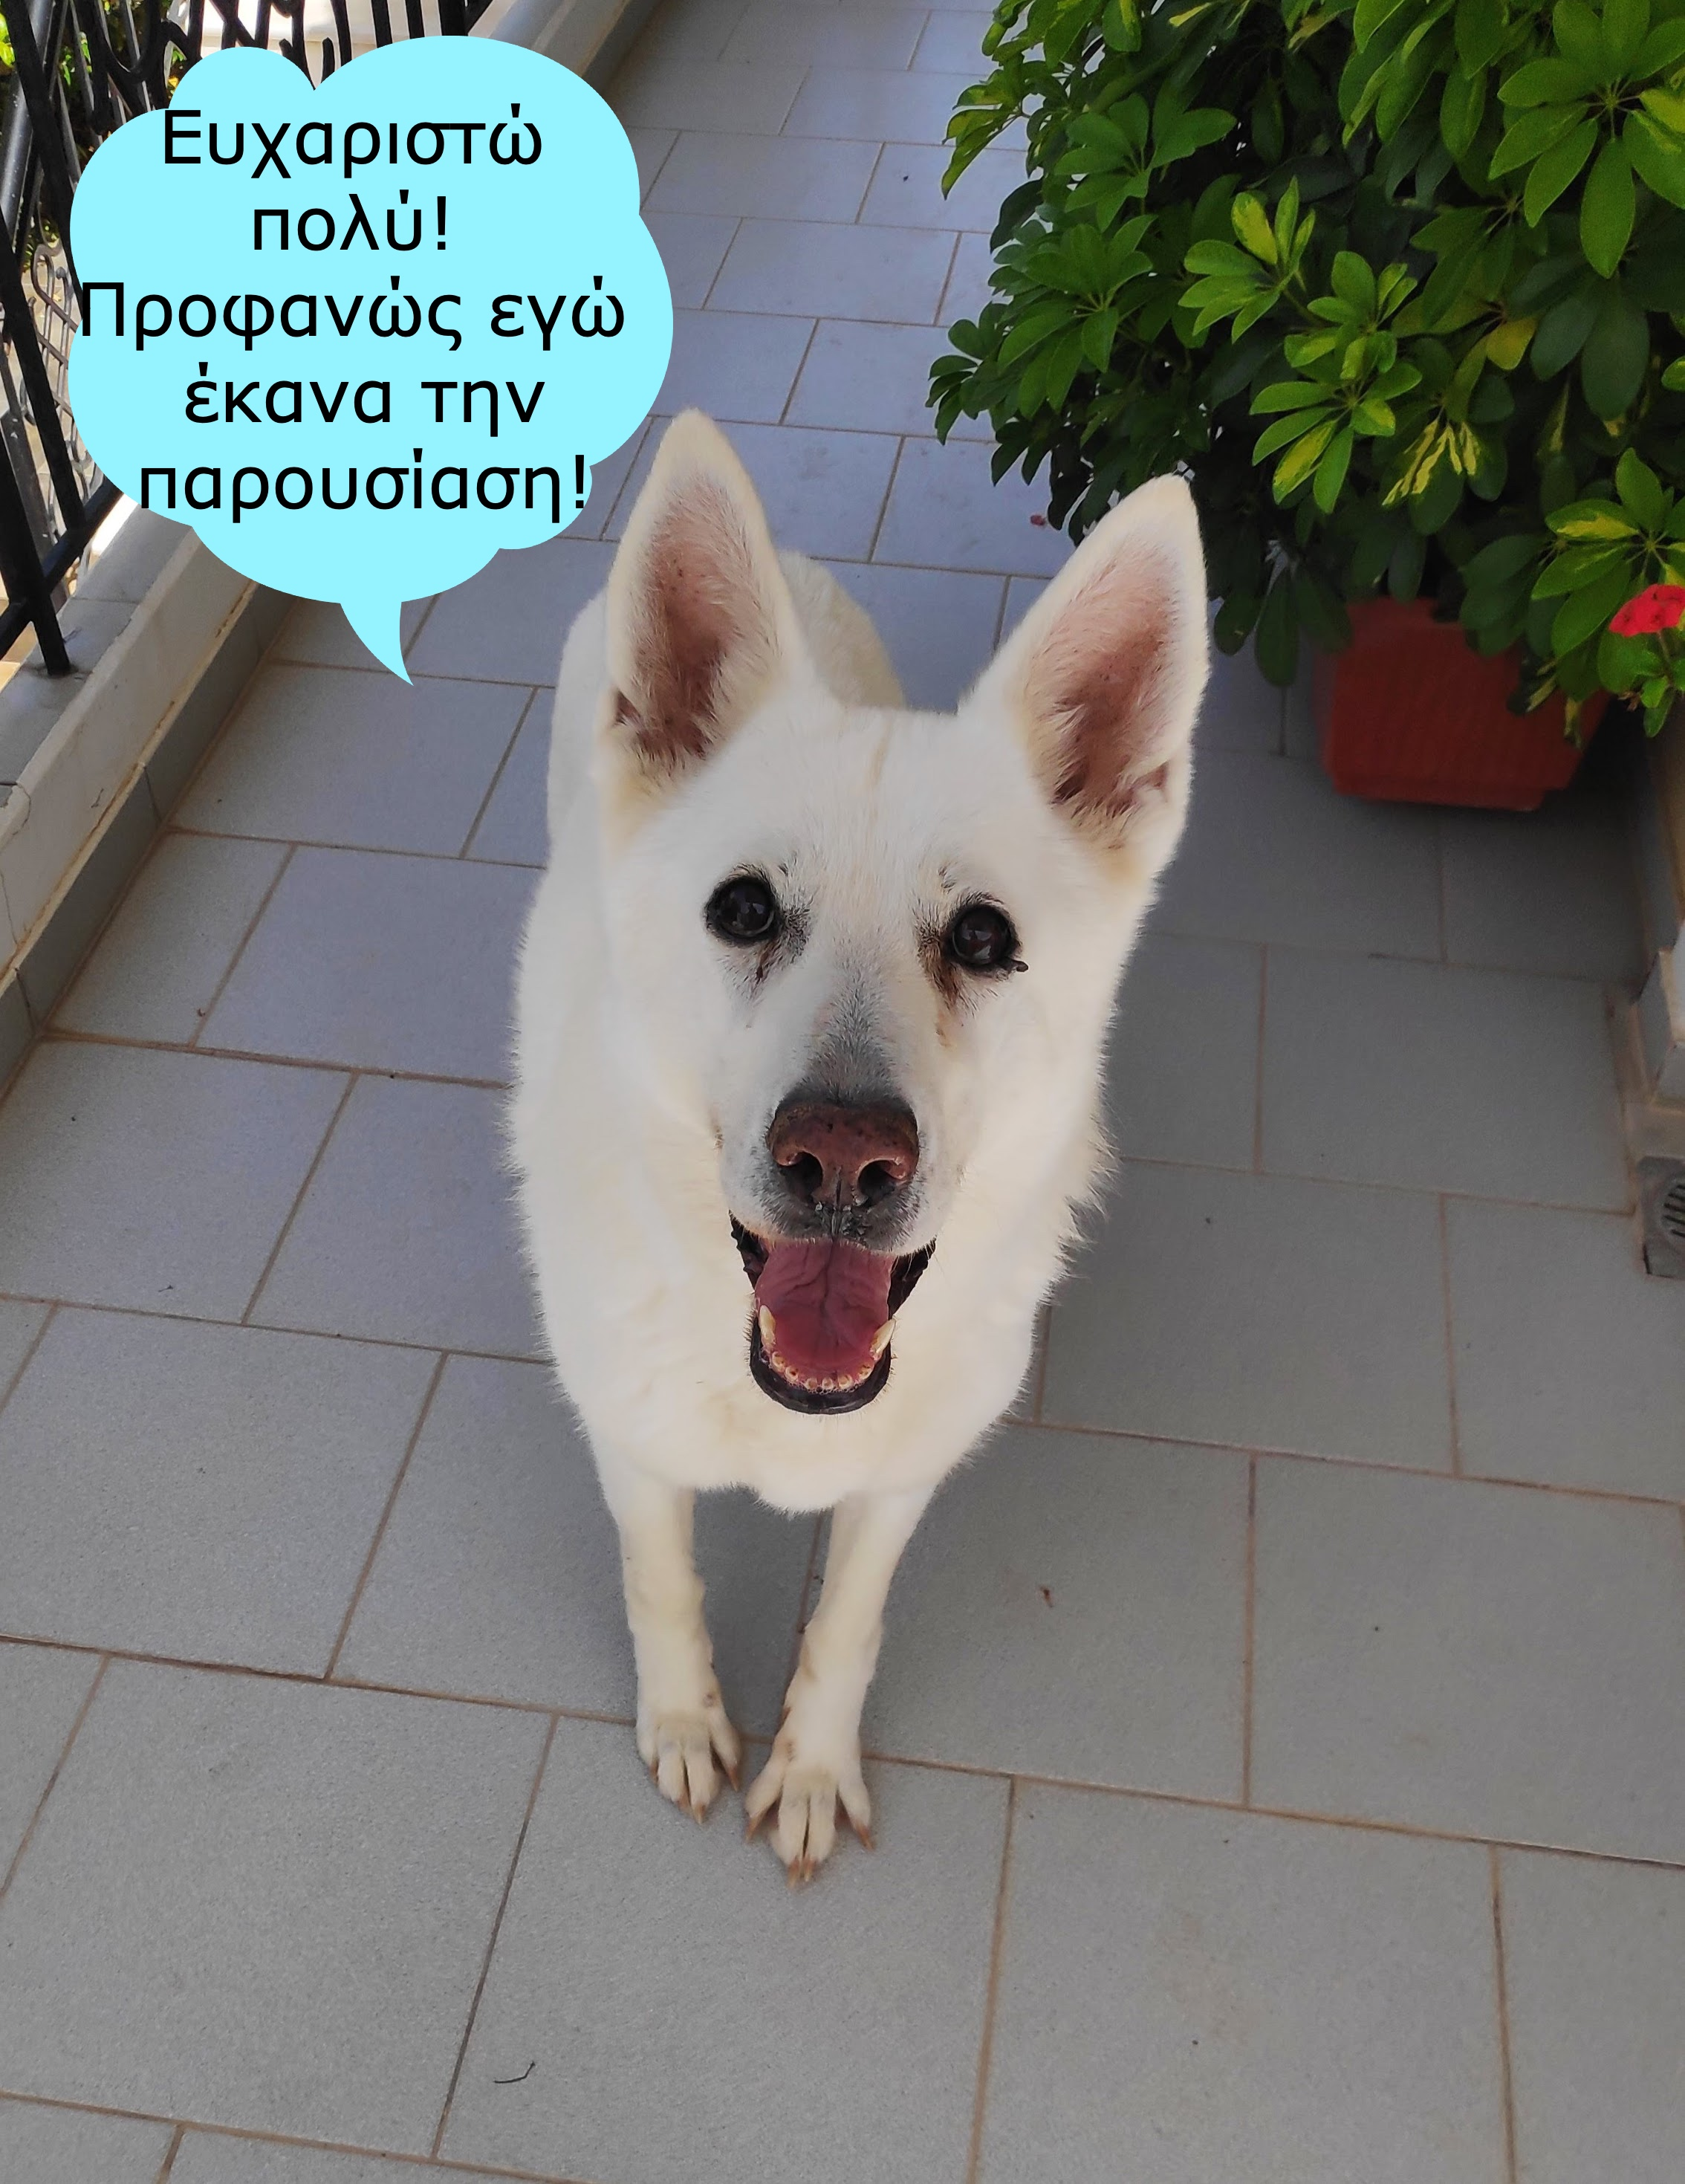
\includegraphics[width=8cm]{Rea1.jpg}
\end{center}
    
\end{frame}

\end{document} 